\documentclass[journal]{IEEEtran}
\usepackage{amsmath,amssymb}
\usepackage{graphicx}
\usepackage{booktabs}
\usepackage[hidelinks,hypertexnames=false]{hyperref}
\hypersetup{
  pdftitle={Collapse-Aware Maintenance of Encrypted Traffic Classifiers under Temporal Drift},
  pdfauthor={Junwei Xiao, Xiaobo Jin, Xiucheng Wu, Zhiquan Liu, Dongjie Liu},
  pdfsubject={Class-aware maintenance of encrypted traffic classifiers under temporal drift}
}
\graphicspath{{./}}
\newcommand{\ours}{CARE}

\begin{document}
\title{Collapse-Aware Maintenance of Encrypted Traffic Classifiers under Temporal Drift}
\author{Junwei Xiao, Xiaobo Jin, Xiucheng Wu, Zhiquan Liu, and Dongjie Liu%
\thanks{Junwei Xiao, Zhiquan Liu, and Dongjie Liu are with the College of Cyber Security, Jinan University, Guangzhou 511443, China (e-mail: xjw20528@stu2024.jnu.edu.cn; zqliu@vip.qq.com; djliu@jnu.edu.cn).}%
\thanks{Xiaobo Jin is with the Department of Intelligent Science, School of Advanced Technology, Xi'an Jiaotong-Liverpool University, Suzhou 215123, China (e-mail: Xiaobo.Jin@xjtlu.edu.cn).}%
\thanks{Xiucheng Wu is with Coremail, Guangzhou 510006, China (e-mail: mwu@coremail.cn).}%
\thanks{Dongjie Liu is the corresponding author.}}
\maketitle

\begin{abstract}
Traffic-based inference supports device management and security monitoring in Internet of Things (IoT) networks, but evolving traffic can make individual classifier outputs unreliable even when aggregate performance appears acceptable. We study a class-asymmetric failure, absorber collapse, in which a previously recognized class loses nearly all recall and its flows are predominantly assigned to other classes. On CESNET-TLS-Year22, 12 of 178 encrypted application classes collapse within nine months; five tested traffic-adapted test-time adaptation methods leave their mean F1 below 0.031. We propose Collapse-Aware Repair (CARE), an operator-reviewed maintenance workflow combining unlabeled class-health monitoring, limited target labeling, all-class historical replay, and head-only repair with distillation. With 1,000 queried labels under strict query-excluded evaluation, CARE raises macro-F1 from 0.629 to 0.700 and collapse-class F1 from 0.028 to 0.332 while retaining stable-class F1 near the static level. A QUIC stress test supports transfer across the evaluated protocol shift. A separate chronological holdout of device-type inference in 11 IoT homes shows recovery of low-recall classes but mixed whole-model outcomes, emphasizing the need to validate candidate updates before deployment.
\end{abstract}
\begin{IEEEkeywords}
Encrypted traffic classification, IoT traffic analytics, concept drift, class collapse, active learning, model maintenance.
\end{IEEEkeywords}

\section{Introduction}
\label{sec:intro}
Long-running IoT traffic analytics can assist device inventory and security monitoring when packet payloads are unavailable. Their predictions are only useful if the classes of operational interest remain recognizable as traffic changes. Residential IoT studies document temporal and cross-home drift in device-type inference~\cite{pashamokhtari2023dynamic,azizi2025labelshift,azizi2026budget}; encrypted application classifiers face related changes in applications and network infrastructure~\cite{soukup2025drift,malekghaini2023drift}. Most evaluations summarize overall accuracy or macro-F1. Such summaries can conceal an individual class whose recall has fallen close to zero.

We call a particular class-asymmetric failure \emph{absorber collapse}: a former class loses recognition and other classes absorb many of its predictions. A maintenance strategy must recover the damaged class without degrading classes that remain useful. This requires a small number of trustworthy target labels because confident predictions on an absorbed victim are themselves wrong. The practical question is therefore not merely whether a classifier adapts to drift, but whether a candidate update improves class-level reliability under a limited annotation budget.

We study this problem first on longitudinal encrypted application traffic, where a fixed taxonomy and month-level partitions support detailed diagnosis. We then examine head repair on a different, real IoT device-type task across 11 households. The application and device labels are distinct; the second study tests the reach of the maintenance idea rather than equating the two tasks. The contributions are: (i) a longitudinal characterization of absorber collapse, (ii) \ours{}, an operator-reviewed workflow for class-health monitoring and label-efficient head repair with all-class preservation, and (iii) strict query-excluded, cross-protocol, and household evaluations that report both recovery and harm.

Three questions organize the evaluation. First, can a class lose nearly all recognition while aggregate metrics remain usable? Second, can a limited verified-label update recover that class without substantially damaging stable ones? Third, how far does this maintenance pattern transfer across target months, protocols, and the different label space of real IoT homes? The TLS analysis addresses the failure and the controlled repair comparison; QUIC tests another encrypted-application protocol; the home study probes device-type maintenance and its variability. We keep these settings separate in the reported conclusions.

\section{Related Work}
Concept drift in encrypted traffic has been documented on CESNET-TLS-Year22 and other longitudinal networks~\cite{soukup2025drift,malekghaini2023drift,jerabek2025eval}. IoT work has studied model selection across homes, changing device priors, and labeling budgets~\cite{pashamokhtari2023dynamic,azizi2025labelshift,azizi2026budget}. These studies motivate maintenance but do not measure the absorber-victim failure and preservation objective considered here.

Label-free test-time adaptation (TTA) methods such as Tent, EATA, SAR, CoTTA, and NOTE~\cite{wang2021tent,niu2022eata,niu2023sar,wang2022cotta,gong2022note} use entropy, confidence, or teacher predictions. Confident absorber errors provide weak corrective signals to these mechanisms. Continual-learning approaches use replay or regularization~\cite{zhu2023iletc,cerasuolo2024memento,kirkpatrick2017ewc,li2018lwf}; our setting instead repairs existing classes in a fixed taxonomy under temporal shift. Active sampling can concentrate a small label budget near uncertain boundaries~\cite{settles2009active,ash2020badge}, while historical reference features and distillation~\cite{hinton2015distilling} can constrain collateral damage. \ours{} combines these established components around a class-level maintenance objective.

There are important distinctions from adjacent tasks. Open-set and class-incremental work, including CPN~\cite{cai2024cpn} and PRIME~\cite{prime2025}, must incorporate previously unseen labels; our label inventory is fixed, and the failure occurs within it. Static long-tail classification~\cite{kang2020decoupling,menon2021longtail} addresses uneven training frequencies, whereas the affected class here was recognizable before its later degradation. Global domain alignment~\cite{ganin2016dann,long2018cdan} can help distribution shift but does not explicitly protect a previously reliable class during a local repair. Traffic-specific active and drift methods such as CADE~\cite{yang2021cade}, ILETC~\cite{zhu2023iletc}, and MEMENTO~\cite{cerasuolo2024memento} address related maintenance problems; we adapt representative controls to the common target-label budget below. The contribution of \ours{} is the failure-specific workflow and its recovery--preservation evaluation, rather than a novel optimizer or selector.

\section{Collapse and Maintenance Method}
\label{sec:method}
\subsection{Failure Definition and Evidence}
Let $f_\phi(x)\in\mathbb{R}^d$ be a frozen feature encoder and $h_\theta$ a $C$-class head trained on source-period data. At a target period $t$, class $c$ is \emph{collapsed} if its recall $R_c^{(t)}<0.1$ with at least 50 test examples. Its primary absorber is $a(c)=\arg\max_{j\ne c}n_{c\to j}$, where $n_{c\to j}$ is the number of true-$c$ flows predicted as $j$. The label budget $B$ is the number of newly queried target labels, not the number of replayed features.

On CESNET-TLS-Year22~\cite{hynek2024cesnet}, a CNN trained on March 2022 (M3) is evaluated through December (M12) over 178 encrypted application classes. Twelve classes fall below the recall threshold by M12. Their largest single absorber receives 13.9--46.1\% of the victim flows. Figure~\ref{fig:collapse} shows abrupt and gradual trajectories: class 56 falls from 0.952 recall in M4 to 0.018 in M5; class 104 declines from 0.629 in M4 to 0.010 by M12. A descriptive Fisher-ratio comparison of victim-absorber feature distributions identifies nine cases of reduced pairwise separation and three with increased separation despite a failing fixed boundary. These signatures motivate target-label repair but do not establish causal mechanisms.

The paired Fisher ratio divides squared between-class feature-mean distance by the sum of within-class spreads. Comparing M4 with M12, nine victim--absorber pairs lose 14--59\% of their ratio, whereas three gain 30--45\% despite continued collapse. The second pattern is consistent with a boundary that no longer fits the shifted feature geometry; it does not prove that the boundary alone caused the error. Both patterns are consequential for a frozen classifier: a detector based only on global accuracy may miss a small victim, and a classifier trained on its own confident pseudo-labels may reinforce the absorber assignment. The observed class-level failure therefore motivates verified target labels together with preservation constraints.

\begin{figure}[!t]
\centering
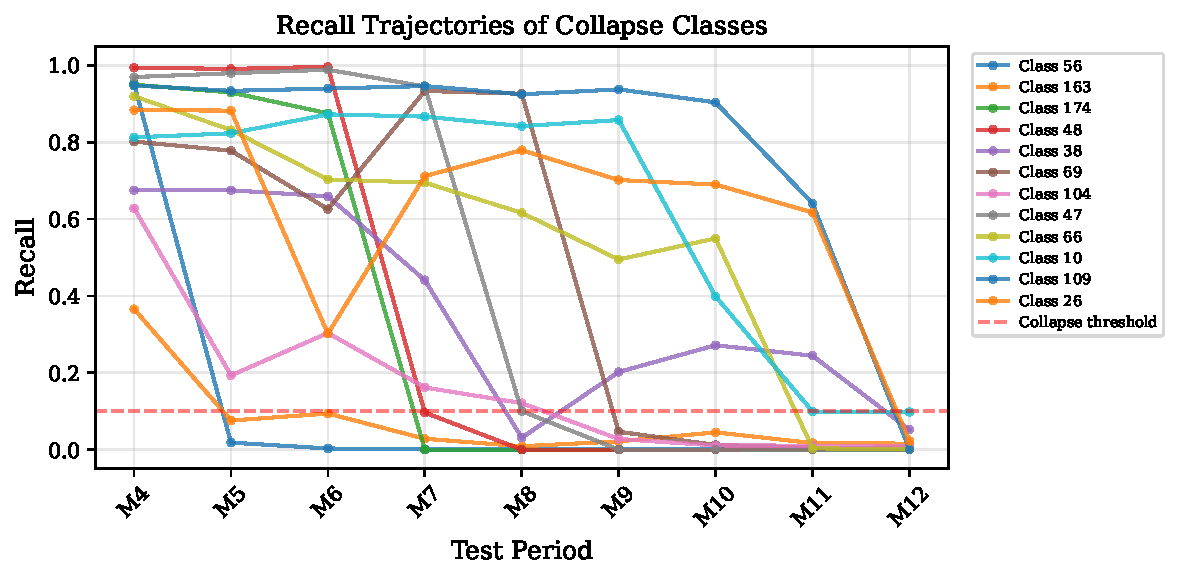
\includegraphics[width=\columnwidth]{fig_collapse_timeline.pdf}
\caption{Recall trajectories of the 12 classes collapsed by M12. The dashed line marks the 0.1 threshold.}
\label{fig:collapse}
\end{figure}

Table~\ref{tab:victims} names all 12 affected classes and their primary absorbers. An absorber need not receive a majority of victim flows: it is the largest destination among several wrong classes. The observed first-collapse months span M5--M12, so a single aggregate M12 score hides both long-standing and late failures. The victim-absorber pair is defined retrospectively from true labels for analysis; the unsupervised monitor below does not have those labels when it scores a target period.

\begin{table}[!t]
\centering
\caption{Collapsed TLS classes at M12. Absorber is the largest incorrect destination; $R$ is victim recall.}
\label{tab:victims}
\scriptsize
\setlength{\tabcolsep}{4pt}
\begin{tabular}{@{}rrrr|rrrr@{}}
\toprule
Victim & Abs. & $R$ & First & Victim & Abs. & $R$ & First\\
\midrule
56 & 96 & .000 & M5 & 163 & 46 & .015 & M5\\
174 & 2 & .000 & M7 & 48 & 14 & .001 & M7\\
38 & 45 & .052 & M8 & 69 & 105 & .005 & M9\\
104 & 2 & .010 & M9 & 47 & 5 & .000 & M11\\
66 & 71 & .001 & M11 & 10 & 156 & .098 & M11\\
109 & 71 & .000 & M12 & 26 & 13 & .022 & M12\\
\bottomrule
\end{tabular}
\end{table}

\subsection{\ours{} Workflow}
Figure~\ref{fig:workflow} places \ours{} beside a deployed classifier. A monitor ranks class risk using unlabeled target predictions relative to a reference period. An operator reviews the alert and authorizes a limited label query. Candidate head repair and validation occur offline; the household study evaluates repair, not a deployed gateway or the complete monitoring workflow.

\begin{figure*}[!t]
\centering
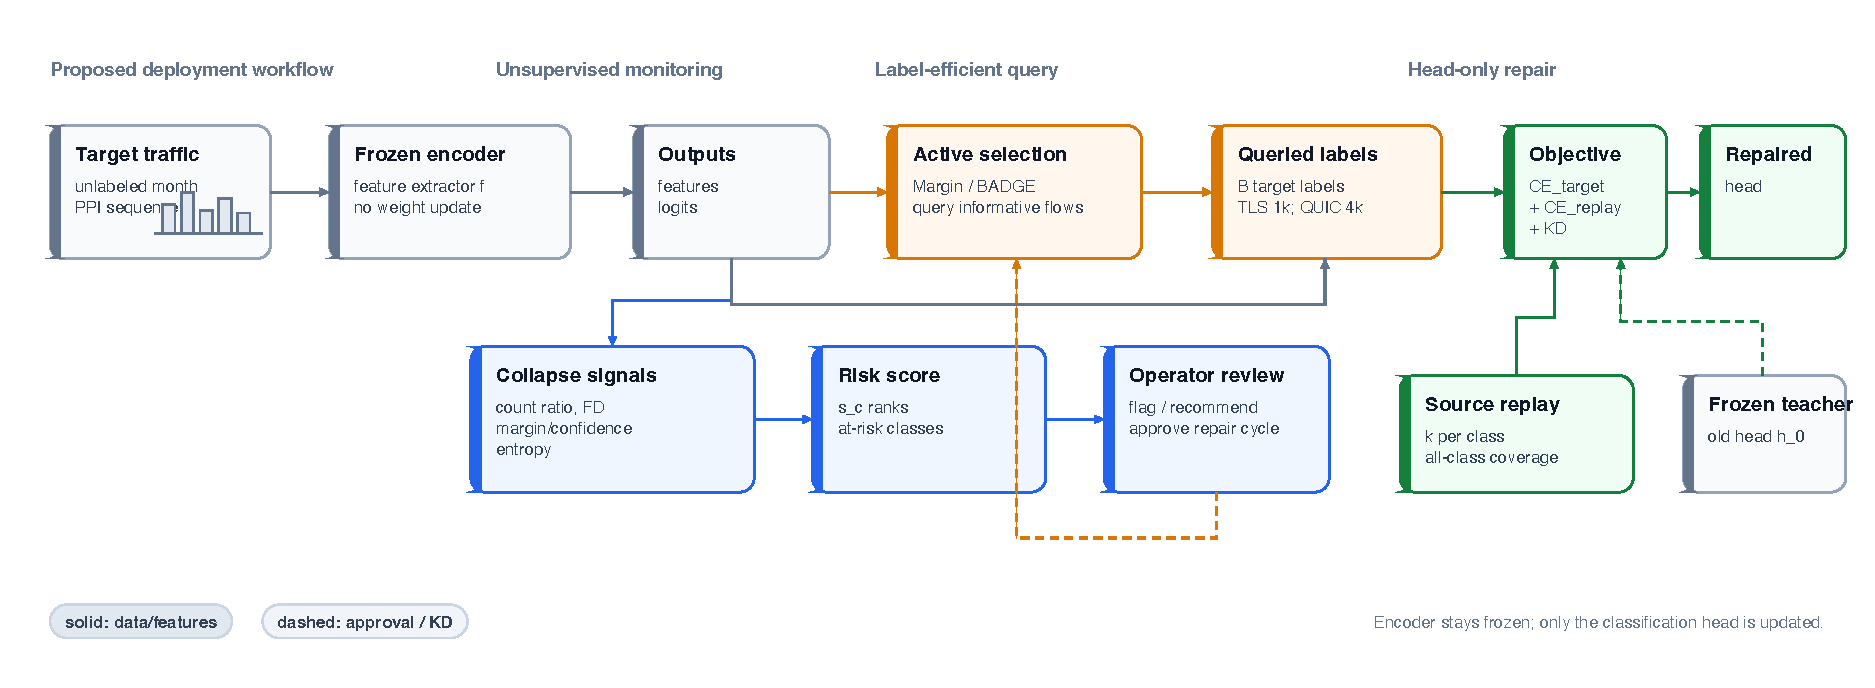
\includegraphics[width=.94\textwidth]{fig_care_workflow_v4.pdf}
\caption{Proposed operator-reviewed maintenance workflow. Monitoring suggests classes for review; approved cycles query target labels and train a candidate head with reference replay and distillation. Deployment and acceptance gates are not evaluated here.}
\label{fig:workflow}
\end{figure*}

For predicted class $c$, the monitor compares target and reference prediction shares $r_c$, feature Fr\'echet distance, and changes in mean logit margin, confidence, and entropy. Median-absolute-deviation normalization puts the latter four signals on comparable scales. The heuristic score is
\begin{equation}
s_c=.40(1-r_c)_+ + .20\tilde d_c+
.15\tilde m_c+.15\tilde q_c+.10\tilde e_c .
\end{equation}
In our diagnostic, $s_c>0.12$ and the 20 highest scores define the review list. These fixed settings are evaluated as a monitor, not as a validated automatic retraining gate. Monitoring does not choose replay classes.

The count ratio uses predicted-class frequencies normalized by the number of flows in each period, so a change in traffic volume alone does not create a count-drop signal. The Fr\'echet term compares frozen feature distributions within predicted regions; the remaining terms track logit behavior. These signals can identify unusual class regions without target ground truth, but they cannot confirm that a true class has collapsed. The operator-reviewed workflow therefore separates alerting from the supervised repair stage. In particular, we retain exemplars from all 178 classes rather than trusting an imperfect alert list to determine which boundaries deserve protection.

After approval, Margin or BADGE~\cite{ash2020badge} selects $B$ target flows for human labeling. The encoder remains frozen. For the default TLS experiment, we add $k=5$ labeled M4 reference features from each of 178 classes (890 total), repeat each queried target feature twice, and initialize the new head from the source head. The objective is $\mathcal L=\mathcal L_{\rm CE}+\lambda\mathcal L_{\rm KD}$, where
\begin{align}
\mathcal L_{\rm CE}
&=\underset{(z,y)\in D_{\rm train}}{\operatorname{mean}}
\ell_{\rm CE}(h_\theta(z),y), \nonumber\\
\mathcal L_{\rm KD}
&=T^2\underset{z\in D_{\rm ref}}{\operatorname{mean}}
D_{\rm KL}\!\left(
\sigma(h_{\theta_0}(z)/T)\Vert
\sigma(h_\theta(z)/T)\right).
\label{eq:loss}
\end{align}
with $\lambda=0.5$ and $T=2$. Distillation applies only to reference features because target-period teacher predictions may contain confident absorber errors. The head uses AdamW~\cite{loshchilov2019adamw} at learning rate $10^{-3}$ for 30 epochs. At $B=1{,}000$, the head sees 2,890 training feature entries but only 1,000 newly labeled target flows.

This update changes only the final linear decision head. Its two supervised sources serve different purposes: queried target labels provide evidence about the current boundary, while reference features keep all historical classes represented in minibatches. Distillation anchors the old head's reference-period output distribution, adding a softer constraint than one-hot replay labels alone. The reference features are stored rather than raw packets in this experiment; we do not claim that feature storage itself supplies a privacy guarantee. BADGE uses top-three-class gradient embeddings compressed to 50 dimensions followed by $B$ k-means++ seeds; Margin uses a global top-two-logit-gap ranking. The selector changes query identities but neither variant receives extra target labels.

\section{Experimental Evaluation}
\label{sec:experiments}
\subsection{Protocol and Main TLS Results}
The primary CESNET-TLS-Year22 experiment uses the DataZoo \texttt{size=S} monthly partitions. The M12 target pool contains 1,323,229 flows. The source CNN has a three-layer 1D convolutional encoder with GroupNorm, a 256-dimensional hidden layer, and a 178-class head; it is trained on M3 packet sizes, directions, and inter-packet times. All active methods query from the target pool, then exclude queried rows from evaluation. We report means and sample standard deviations over five repair seeds with one fixed source checkpoint. Collapse F1 averages the 12 M12 static-collapse classes; stable F1 averages a fixed 20-class post-hoc preservation set. The CESNET exporter update around week 10~\cite{hynek2024cesnet} is shared by compared methods but limits attribution of all drift to applications.

\begin{table}[!t]
\centering
\caption{M12 TLS results under strict query exclusion. Active rows use 1,000 labels, all-class replay, and KD (five repair seeds); TTA rows use no labels.}
\label{tab:main}
\scriptsize
\setlength{\tabcolsep}{3pt}
\begin{tabular}{@{}lcccc@{}}
\toprule
Method & Macro-F1 & Collapse F1 & Stable F1 & \#Col.\\
\midrule
Static & .629 & .028 & .903 & 12\\
Tent & .631 & .026 & .903 & 12\\
EATA & .629 & .028 & .903 & 12\\
SAR & .629 & .026 & .901 & 11\\
CoTTA & .630 & .027 & .903 & 12\\
NOTE & .630 & .027 & .902 & 12\\
\midrule
Entropy + replay/KD & $.628\!\pm\!.004$ & $.078\!\pm\!.015$ & $.887\!\pm\!.004$ & 10.2\\
Coreset + replay/KD & $.633\!\pm\!.005$ & $.116\!\pm\!.042$ & $.886\!\pm\!.007$ & 8.8\\
Random + replay/KD & $.668\!\pm\!.004$ & $.188\!\pm\!.024$ & $.892\!\pm\!.006$ & 8.2\\
\ours{}-Margin & $.686\!\pm\!.001$ & $.256\!\pm\!.009$ & $.892\!\pm\!.003$ & 5.8\\
\textbf{\ours{}-BADGE} & $\mathbf{.700\!\pm\!.003}$ & $\mathbf{.332\!\pm\!.040}$ & $\mathbf{.894\!\pm\!.004}$ & 4.0\\
\bottomrule
\end{tabular}
\end{table}

Table~\ref{tab:main} shows that \ours{}-BADGE has the highest mean macro-F1 and collapse F1 among the evaluated repair rows, while stable F1 remains close to the static level. Under our traffic-adapted implementations, five TTA variants leave collapse F1 below .031; EATA, CoTTA, and NOTE involve packet-sequence-specific simplifications, so this is evidence about the tested versions. A separate seed-matched untouched 20\% M12 holdout compares a Chen-inspired high-confidence pseudo-label update~\cite{chen2025selfevolving}, not an exact reproduction. Its best-macro sensitivity setting reaches .614 macro-F1 and .014 collapse F1, versus .701 and .310 for \ours{}-BADGE; the methods use different supervision and update budgets. Same-budget drift and continual-learning controls reach at most .678 macro-F1 (MEMENTO~\cite{cerasuolo2024memento}) or .307 collapse F1 (an expanded-head control), with lower stable F1 than \ours{}-BADGE. Full implementation details and seed-wise records are in Supplementary Material S1.

The average across 12 victims does not imply universal recovery. Table~\ref{tab:classrecovery} makes this variation explicit. Class 56 recovers strongly under both selectors, but class 109 stays at zero F1; class 174 favors Margin, whereas classes 47 and 10 favor BADGE in this run. Mean labels assigned directly to a victim are often only a few of the 1,000 queries. Thus some improvements can come from changing boundaries using other labeled target classes plus all-class replay. Selecting more labels from a particular victim is not sufficient evidence that it will recover.

\begin{table*}[!t]
\centering
\caption{Per-victim M12 results under strict query exclusion ($B=1{,}000$, five seeds). $n$ is static test support; selected is the mean number of paid true-class labels. F1 values are seed means.}
\label{tab:classrecovery}
\scriptsize
\setlength{\tabcolsep}{3.8pt}
\begin{tabular}{@{}rrrrrrrr@{}}
\toprule
Victim & Abs. & $n$ & Static F1 & Margin F1 & BADGE F1 & Margin selected & BADGE selected\\
\midrule
56  & 96  & 12137 & .001 & .784 & .829 & 12.0 & 13.6\\
163 & 46  & 1741  & .026 & .168 & .235 & 3.0 & 4.8\\
174 & 2   & 1507  & .000 & .262 & .044 & 4.0 & 1.6\\
48  & 14  & 3361  & .002 & .568 & .767 & 4.0 & 4.8\\
38  & 45  & 193   & .090 & .410 & .210 & 3.0 & 1.2\\
69  & 105 & 1866  & .008 & .042 & .177 & 3.0 & 2.4\\
104 & 2   & 1744  & .016 & .664 & .594 & 8.0 & 3.6\\
47  & 5   & 618   & .000 & .004 & .462 & 0.0 & 2.2\\
66  & 71  & 1955  & .002 & .002 & .144 & 1.0 & 4.2\\
10  & 156 & 1004  & .162 & .121 & .441 & 0.0 & 1.8\\
109 & 71  & 393   & .000 & .000 & .000 & 0.0 & 1.6\\
26  & 13  & 807   & .025 & .046 & .087 & 1.0 & 2.6\\
\midrule
Mean & & & .028 & .256 & .332 & & \\
\bottomrule
\end{tabular}
\end{table*}

Table~\ref{tab:cl} separates the same-budget supervised controls from the label-free TTA rows. CADE-score~\cite{yang2021cade} substitutes a drift-score selector; ILETC~\cite{zhu2023iletc} uses synthetic or real replay without KD; MEMENTO~\cite{cerasuolo2024memento} fine-tunes the full model with KD; the expanded-head control increases capacity. All labeled rows use 1,000 target labels and strict query exclusion. Except for CADE-score and \ours{}-BADGE, they use the same Margin query batch. Consequently, the table compares implemented maintenance strategies, not an isolated causal effect of any single component.

\begin{table}[!t]
\centering
\caption{Same-budget M12 drift and continual-learning controls (five seeds). CARE rows are repeated from Table~\ref{tab:main}.}
\label{tab:cl}
\scriptsize
\setlength{\tabcolsep}{3pt}
\begin{tabular}{@{}lccc@{}}
\toprule
Method & Macro-F1 & Collapse F1 & Stable F1\\
\midrule
CADE-score & $.637\!\pm\!.004$ & $.118\!\pm\!.015$ & $.889\!\pm\!.003$\\
ILETC-GAN & $.650\!\pm\!.004$ & $.219\!\pm\!.010$ & $.851\!\pm\!.009$\\
ILETC-real & $.659\!\pm\!.003$ & $.236\!\pm\!.010$ & $.854\!\pm\!.016$\\
Expanded head & $.673\!\pm\!.003$ & $.307\!\pm\!.005$ & $.871\!\pm\!.008$\\
MEMENTO & $.678\!\pm\!.002$ & $.255\!\pm\!.005$ & $.892\!\pm\!.004$\\
\ours{}-Margin & $.686\!\pm\!.001$ & $.256\!\pm\!.009$ & $.892\!\pm\!.003$\\
\ours{}-BADGE & $.700\!\pm\!.003$ & $.332\!\pm\!.040$ & $.894\!\pm\!.004$\\
\bottomrule
\end{tabular}
\end{table}

\noindent\emph{Evaluation sensitivity.}
For the Chen-inspired comparison, each seed reserves 264,645 of the 1,323,229 M12 flows as an untouched 20\% holdout before any adaptation. The pseudo-label baseline updates encoder and head with confident target predictions and no human labels; its $.614$ macro-F1 setting was chosen post hoc from a threshold sweep. \ours{} uses 1,000 verified labels and a frozen encoder. This comparison tests failure-mode behavior on matched holdouts rather than equal supervision. In the main strict experiment, paired $t$-tests favor Margin over Random and BADGE over Margin, but the exact two-sided Wilcoxon test with five seeds cannot reach $p<.05$ (minimum $p=.0625$); selector rankings therefore remain exploratory.

\subsection{Components, Drift Periods, and Monitoring}
Table~\ref{tab:components} reports the core component bundles. Replay and KD together retain substantially more stable-class F1 than target-only fine-tuning, while full \ours{} improves both macro and collapse F1 at this operating point. These bundles differ in target repetition or replay coverage, so their differences do not isolate individual loss terms; Supplementary Material S2 provides separate matched-update reconstruction controls and qualifies the incremental effect of reference cross-entropy.

\begin{table}[!t]
\centering
\caption{M12 component bundles (Margin queries, strict evaluation, five seeds). FT: target fine-tuning; Rpl: all-class replay; KD: reference distillation.}
\label{tab:components}
\scriptsize
\setlength{\tabcolsep}{4pt}
\begin{tabular}{@{}lccc@{}}
\toprule
Configuration & Macro-F1 & Collapse F1 & Stable F1\\
\midrule
Static & .629 & .028 & .903\\
FT only & $.638\!\pm\!.000$ & $.134\!\pm\!.001$ & $.839\!\pm\!.001$\\
FT + Rpl & $.659\!\pm\!.003$ & $.236\!\pm\!.010$ & $.854\!\pm\!.016$\\
FT + KD (targeted replay) & $.670\!\pm\!.000$ & $.152\!\pm\!.007$ & $.887\!\pm\!.004$\\
Full \ours{} & $.686\!\pm\!.001$ & $.256\!\pm\!.009$ & $.892\!\pm\!.003$\\
\bottomrule
\end{tabular}
\end{table}

\noindent\emph{Budget and replay coverage.}
Figure~\ref{fig:budget} reports the original Margin budget sweep. At 2,000 paid labels, collapse F1 reaches $.437\pm.004$ and the number of the 12 predefined victims still below .1 recall falls from 12 to two. At 8,000 labels, collapse F1 reaches $.609\pm.007$. Stable F1 remains at least .887 across tested positive budgets, compared with .903 for static. The 1,000-label point used for baseline comparisons is therefore a constrained operating point rather than a claim that this is the optimal budget. Query labels comprise only .076\% of the 1,323,229-flow M12 target pool at that point, though the experiment does not measure human labeling time.

\begin{figure*}[!t]
\centering
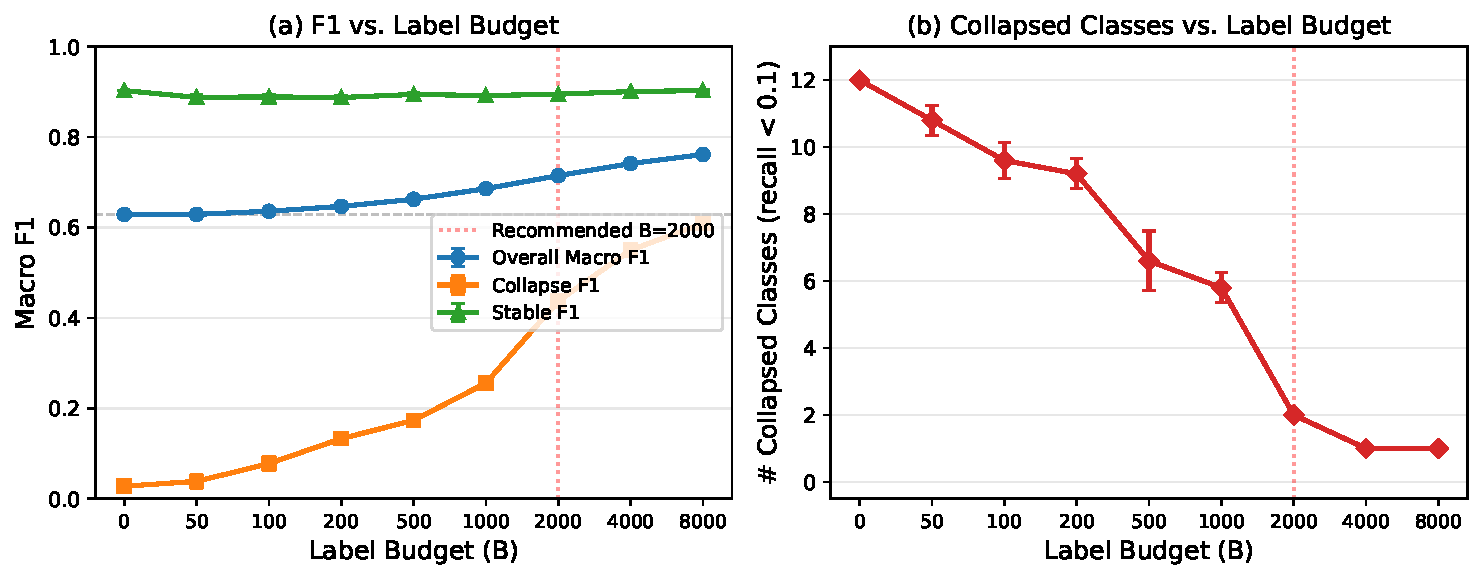
\includegraphics[width=.86\textwidth]{budget_curve.pdf}
\caption{Margin-query budget sweep on M12 TLS, with five repair seeds. Dashed lines mark the static model; the right panel counts predefined M12 victims that remain below .1 recall.}
\label{fig:budget}
\end{figure*}

The replay comparison in Table~\ref{tab:replay} changes coverage while holding the 1,000-label Margin batch fixed. All-class replay with five features per class has higher mean macro and collapse F1 than targeted replay using approximately the same number of features. The targeted subset is an oracle stable-plus-absorber list, so its result is a favorable control for narrow replay rather than a deployable selector. All-class replay with one feature per class also exceeds targeted replay in macro-F1 despite using fewer stored features. This supports broad class coverage in the tested configuration; it does not establish a general optimal replay size.

\begin{table}[!t]
\centering
\caption{M12 replay strategies ($B=1{,}000$, Margin, five seeds). Targeted replay uses an oracle class list.}
\label{tab:replay}
\scriptsize
\setlength{\tabcolsep}{4pt}
\begin{tabular}{@{}lccc@{}}
\toprule
Reference features & Count & Macro-F1 & Collapse F1\\
\midrule
All-class, 5/class & 890 & $.686\pm.001$ & $.256\pm.009$\\
Targeted, 30/class & $\sim900$ & $.678\pm.001$ & $.243\pm.003$\\
All-class, 1/class & 178 & $.680\pm.003$ & $.231\pm.015$\\
\bottomrule
\end{tabular}
\end{table}

Under the same 1,000-label Margin budget, full encoder-and-head fine-tuning achieves $.678\pm.001$ macro-F1 and $.256\pm.005$ collapse F1, versus $.686\pm.001$ and $.256\pm.009$ for head-only repair. The nearly identical collapse result and lower macro-F1 make the smaller head update a reasonable maintenance choice at this budget, without ruling out encoder changes when representations are irrecoverably mixed.

Table~\ref{tab:period} evaluates the same Margin query budget at four target months. The fixed collapse set is defined from the M12 static model; thus its earlier-month F1 is a consistent longitudinal endpoint, not an assertion that all 12 classes had already collapsed. Both macro and fixed-set F1 improve at every tested month. Earlier repair has higher fixed-set F1, but sequential deployment and repeated maintenance are not tested.

\begin{table}[!t]
\centering
\caption{TLS temporal results, $B=1{,}000$, Margin, three repair seeds. Col. is the fixed 12-class M12 collapse set.}
\label{tab:period}
\scriptsize
\setlength{\tabcolsep}{4pt}
\begin{tabular}{@{}lcccc@{}}
\toprule
Period & Static macro & CARE macro & Static col. & CARE col.\\
\midrule
M7 & .740 & $.776\!\pm\!.003$ & .503 & $.633\!\pm\!.028$\\
M9 & .691 & $.739\!\pm\!.003$ & .280 & $.392\!\pm\!.005$\\
M11 & .649 & $.708\!\pm\!.002$ & .145 & $.408\!\pm\!.016$\\
M12 & .629 & $.686\!\pm\!.002$ & .028 & $.255\!\pm\!.012$\\
\bottomrule
\end{tabular}
\end{table}

The unlabeled detector is evaluated separately from the repair tables. Table~\ref{tab:detect} gives review-list quality for the 20 highest-risk classes. Detection ground truth uses retrospective recall below .1 and support at least 50; those labels are used only for scoring. At M12, the full five-signal detector retrieves 10 of 12 collapsed classes, with precision .50 and recall .833. A count-drop and Fr\'echet-distance-only variant reaches precision .45 and recall .75 at M12, so the full score improves this tested operating point. However, the detector threshold and weights have not been calibrated on an independent deployment.

\begin{table}[!t]
\centering
\caption{Unlabeled monitoring diagnostic over TLS target months. GT is the number of retrospective collapsed classes; $k=20$ review candidates.}
\label{tab:detect}
\scriptsize
\setlength{\tabcolsep}{5pt}
\begin{tabular}{@{}lrrrr@{}}
\toprule
Period & GT & Precision & Recall & F1\\
\midrule
M7 & 5 & .200 & .800 & .320\\
M9 & 8 & .350 & .875 & .500\\
M11 & 10 & .450 & .900 & .600\\
M12 & 12 & .500 & .833 & .625\\
\bottomrule
\end{tabular}
\end{table}

\subsection{QUIC and IoT Settings}
On CESNET-QUICEXT-25 XS~\cite{cesnetquicext25,mucke2025waiting}, we train on M-2024-6 and evaluate on M-2025-5 over 44 classes. Three drift-induced classes collapse. Static macro/collapse F1 is .502/.049. \ours{}-Margin with 1,000 queried labels reaches $.564\pm.003$ / $.114\pm.002$; \ours{}-BADGE with 4,000 labels reaches $.586\pm.007$ / $.191\pm.030$ under strict query exclusion (five seeds). The stronger result uses a larger label budget and defines a distinct operating point.

Table~\ref{tab:quic} gives the intermediate budgets. Class 21 has near-zero target recall but is omitted from the three drift-induced victims because the source model already failed to learn it in the reference period. The budget response differs from TLS: at 1,000 labels, Margin gives stronger collapse recovery than BADGE in this dataset, while BADGE has the higher mean at 4,000 labels. Cross-protocol transfer therefore concerns the overall repair pattern and is not evidence for a universally best selector or budget.

\begin{table}[!t]
\centering
\caption{QUICEXT-25 XS stress test, M-2024-6 to M-2025-5, strict query exclusion (five seeds).}
\label{tab:quic}
\scriptsize
\setlength{\tabcolsep}{3pt}
\begin{tabular}{@{}lrrcc@{}}
\toprule
Method & $B$ & Macro-F1 & Collapse F1 & \#Col.\\
\midrule
Static & 0 & .502 & .049 & 3.0\\
Margin & 1000 & $.564\pm.003$ & $.114\pm.002$ & 2.0\\
BADGE & 1000 & $.563\pm.006$ & $.091\pm.017$ & 2.8\\
Margin & 2000 & $.577\pm.003$ & $.126\pm.014$ & 2.0\\
BADGE & 2000 & $.578\pm.006$ & $.144\pm.031$ & 2.2\\
Margin & 4000 & $.578\pm.002$ & $.132\pm.021$ & 1.8\\
BADGE & 4000 & $.586\pm.007$ & $.191\pm.030$ & 1.2\\
\bottomrule
\end{tabular}
\end{table}

For a device-type task, we use the public residential IoT flow archive~\cite{pashamokhtari2023dynamic}. Its official inventory maps MAC addresses to 24 known device types; MAC addresses, IP addresses, ports, timestamps, and labels are excluded from input features. For each of 11 homes with all types in the source window, observed days are split chronologically into source, query, development, and untouched final windows at approximately 50\%, 70\%, and 85\% of days. Home10 lacks two source types and is excluded from this fixed-vocabulary comparison. A separate source MLP uses flow statistics and protocol indicators. Each of five overlapping repair seeds per home pays for 1,000 uniformly sampled query labels; the ported \ours{} head uses those labels and five source reference features per class. After examining development outcomes, we froze final-window predictions and compared static, target-only update, \ours{}, and fixed 0.5 source/target head interpolation (BCWI) before scoring final labels. This mixed-protocol study tests head repair without the monitoring or BADGE stages.

\begin{table}[!t]
\centering
\caption{IoT device-type final-window holdout, 11 homes. Macro-F1 averages device types present in each home's final window; CARE and BCWI average five overlapping seeds. Homes are the independent units.}
\label{tab:iot}
\scriptsize
\setlength{\tabcolsep}{4pt}
\begin{tabular}{@{}lrrrr@{}}
\toprule
Home & Static & CARE & BCWI & CARE $\Delta$ (pp)\\
\midrule
01 & .5895 & .6100 & .6106 & $+2.047$\\
02 & .4623 & .4606 & .4915 & $-0.172$\\
03 & .5201 & .5171 & .5421 & $-0.306$\\
04 & .4327 & .4444 & .4539 & $+1.163$\\
05 & .4498 & .4332 & .4636 & $-1.661$\\
06 & .5470 & .4829 & .5109 & $-6.410$\\
07 & .5536 & .5009 & .4603 & $-5.272$\\
08 & .4930 & .5214 & .5429 & $+2.838$\\
09 & .5564 & .5687 & .6095 & $+1.234$\\
11 & .5553 & .5593 & .5511 & $+0.399$\\
12 & .5609 & .5379 & .5780 & $-2.293$\\
\midrule
Mean & .5201 & .5124 & .5286 & $-0.767$\\
\bottomrule
\end{tabular}
\end{table}

The holdout results in Table~\ref{tab:iot} are mixed: \ours{} improves whole-model macro-F1 in five homes and reduces equal-home mean macro-F1 by .767 percentage points (.52006 to .51239), while BCWI reaches .52858. Yet low-recall device-type mean F1 increases from .03988 to .13887 under \ours{}; on average .78 of 1.64 qualifying low-recall types per home regain at least .1 recall. Among an average 5.55 stable-recognition types per home, .42 lose over five F1 points; the conditional negative-flip rate is .05908. No home-type pair satisfies the stricter incident-collapse condition of high development recall followed by near-zero final recall. Thus the household study supports class-level recovery under a different label space but not consistent whole-model improvement. Supplementary Material S3 supplies the frozen protocol, per-home and per-class results, and per-row predictions.

The group definitions were fixed before final-window labels were read. A low-recall type has at least 50 final rows and static recall below .1; a stable-recognition type has at least 50 rows and static recall at least .8. These are retrospective evaluation groups, not inputs to query selection or model routing. Table~\ref{tab:iotgroups} distinguishes recovery from harm across the four final-window methods. CARE has the highest mean low-recall F1 and the most recovered types, while the simple interpolation control has higher whole-model F1 and fewer stable-class losses. The descriptive 95\% home-bootstrap interval for the CARE-minus-static equal-home macro-F1 difference is $[-2.474,0.756]$ percentage points. The five paid-label seeds share homes, so the home is the unit of replication.

\begin{table}[!t]
\centering
\caption{Final-window IoT class-level outcomes, equal-home means. Recovered counts are per home among 1.64 low-recall types on average; stable losses are per home among 5.55 stable types. NFR is conditional on static-correct rows.}
\label{tab:iotgroups}
\scriptsize
\setlength{\tabcolsep}{3pt}
\begin{tabular}{@{}lcccc@{}}
\toprule
Method & Low F1 & Recovered & Stable loss & NFR\\
\midrule
Static & .040 & 0 & 0 & 0\\
Target-only & .103 & .55 & .73 & .123\\
CARE & .139 & .78 & .42 & .059\\
BCWI 0.5 & .104 & .49 & .29 & .048\\
\bottomrule
\end{tabular}
\end{table}

Cross-home variation is material: CARE's macro-F1 gains range from $+2.838$ points in home08 to $-6.410$ in home06. In the examined development windows, 17 home--type pairs met a related low-recall criterion; CARE increased mean F1 for all 17, but 12 had fewer than five paid positives on average. Across all 246 present home--type pairs, 124 improved, 120 declined, and two were unchanged. These development observations informed the final endpoints and cannot serve as an independent test of a route chosen from them. Three preselected descriptive associations between final CARE gain and class-share shift, maximum class share, or paid-positive coverage are weak ($\rho=.027,-.345,-.012$ over 11, 11, and 10 homes). They do not yet explain which deployment will benefit. The final results therefore support class-aware acceptance checks rather than a claim that CARE reliably improves every home.

\section{Discussion and Conclusion}
Encrypted application traffic provides strong evidence for the class-asymmetric failure and for label-efficient recovery under the specified protocol. The separate IoT test shows why a device-management deployment cannot select updates solely from an average gain or a recovered type: another type or home may be harmed. An operational use of \ours{} would require class-health review, an affordable label budget, and a predeployment acceptance check. Neither a live gateway nor an acceptance gate was evaluated.

The empirical mechanism is a maintenance mismatch. In the TLS experiment, the model remains useful for many classes while 12 fall below .1 recall; a global score gives limited guidance about which class needs attention. The tested label-free TTA variants barely change the victim F1, consistent with confident misclassification providing no corrective target signal. Verified labels make boundary movement possible, while replay and reference distillation constrain movement on other classes. The component and replay comparisons support this combined design at the reported budget, although they do not isolate a unique causal contribution for every loss term. The failure of class 109 to recover in Table~\ref{tab:classrecovery} also marks a practical boundary: a small head update is not guaranteed to repair every representation.

For IoT analytics, the relevant maintenance unit may be a device type rather than an encrypted application class. The same reliability question nevertheless arises when an operator relies on per-type recognition for inventory, troubleshooting, or security review. The 11-home result is informative precisely because it changes the data source, feature representation, and label taxonomy. CARE raises mean F1 for low-recall types in the final window, while its aggregate gain varies by home and is negative on average. A candidate maintenance update should therefore be checked for both recovered and damaged types in the deployment where it will run. Figure~\ref{fig:workflow} presents that as an operator-reviewed sequence: monitor, obtain labels, fit a candidate head, validate class-level effects, and only then consider activation. The present experiments evaluate the monitor and repair stages separately; they do not measure an integrated live system.

The annotation budget is small as a fraction of the TLS target pool, but labeling 1,000 flows may still be costly in practice. Margin is computationally simpler than BADGE and gives lower mean recovery in the main TLS table; BADGE's stronger mean result requires the more expensive gradient-embedding selection. In the matched timing audit, the full BADGE program takes $166.6\pm8.2$ seconds versus $48.5\pm0.8$ seconds for Margin on one NVIDIA L20. The choice is therefore an operating decision conditioned on review capacity, compute, and the value of recovering a particular class. For a scheduled maintenance job, storing a small set of reference features and updating only the head offers a bounded update path, subject to privacy and validation requirements at the actual site.

The main limitations are one primary source checkpoint for the principal TLS table, an endpoint-defined stable set, traffic-adapted TTA implementations, and different architectures, features, selectors, and schedules in the IoT port. The CESNET source period also contains an exporter change. These conditions limit causal attribution and generalization. The present contribution is a class-aware maintenance framework, supported by substantial collapse recovery in encrypted application traffic and bounded by heterogeneous outcomes in IoT device-type inference.

\section*{Funding}
This research did not receive any specific grant from funding agencies in the public, commercial, or not-for-profit sectors.

\section*{Data and Code Availability}
The public datasets are CESNET-TLS-Year22~\cite{hynek2024cesnet} (\url{https://doi.org/10.5281/zenodo.10608607}), CESNET-QUICEXT-25~\cite{cesnetquicext25} (\url{https://doi.org/10.5281/zenodo.17249078}), and the residential IoT flow archive~\cite{pashamokhtari2023dynamic} (\url{https://iotanalytics.unsw.edu.au/homedataset.html}). Supplementary Material S1 contains implementation files and archived CESNET experiment records. The original exact size-S row identities and full feature caches are unavailable, so S1 does not support complete end-to-end reruns of every original experiment. S2 documents the independently reconstructed component controls, whose records are included in S1. S3 contains the 11-home final-window protocol, tables, predictions, code, and file hashes; public raw IoT flows are required to rescore predictions. S1, S2, and S3 are separate supplementary files with this submission.

\section*{Acknowledgment}
OpenAI Codex assisted with language editing throughout the manuscript and with figure rendering from archived records in the Collapse and Maintenance Method section. It also assisted with code implementation and result verification for the IoT device-type study in the Experimental Evaluation section and the reconstruction controls in Supplementary Material S2. The authors reviewed the generated text, code, figures, and results and take responsibility for the accuracy and integrity of the article.

\bibliographystyle{IEEEtran}
\bibliography{references}
\end{document}
